% This file should be replaced with your file with an thesis content.
%=========================================================================
% Authors: Michal Bidlo, Bohuslav Křena, Jaroslav Dytrych, Petr Veigend and Adam Herout 2019

% For compilation piecewise (see projekt.tex), it is necessary to uncomment it and change
% \documentclass[../projekt.tex]{subfiles}
% \begin{document}

\chapter{Introduction}

This text serves as example content of this template and as a recap of the most important information from regulations, it also provides additional useful information, that you will need when you write a technical report for your academic work. Check out appendix \ref{jak} before you use this template as it contains vital information on how to use it.

Even though some students only need to know and comply with the official formal requirements stated in regulations as well as typographical principles to write a good diploma thesis (bachelor's thesis is a diploma thesis too -- you get a diploma for it), it is never a~bad idea to familiarize yourself with some of the well-established procedures for writing a~technical text and make things easier for yourself. Some supervisors had prepared breakdowns of proven procedures that have lead to tens of successfully presented academic works. A~selection of the most interesting procedures available to the authors of this work at the time of writing can be found in chaptes below. If your supervisor has their own web page with recommended procedures, you can skip these chapters and follow their instructions instead. If that is not the case, you should read the respective chapters proir to consulting your supervisor about the structure and contents of your academic work.

Diploma thesis is an extensive work and the technical report should reflect it. It is not easy for everyone to sit down and simply write it. You need to know where to begin and how to progress. One of many viable approaches is to start with keywords and abstract, this helps you establish what the most important part of your work is. More on that in~chapter~\ref{abstrakt}.

Once the abstract is finished, you can start with the text of the technical report. The first thing you should do is create a structure for your work, that you'll later fill with text. Chapter \ref{struktura} provides basic information and hints on writing a technical text, that can help you avoid mistakes beginners make, create chapter titles and figure out what the approximate length of individual chapters should be. The chapter concludes with an approach that should make writing a thesis much easier.

Diploma theses in the field of information technology have a specific  structure. The introduction is followed by a chapter or chapters dealing with the summary of the current state. The next chapter should evaluate the current state and provide a solution, that will be implemented and tested. The conclusion should contain evaluated results and ideas for future development. Even though the chapter titles and their length may differ from other theses, you can always find chapters that correspond with this structure. Chapter \ref{kapitoly} deals with the contents of chapters that commonly occur in dimploma theses in the field of information technology. Most students will only use a subset of all the described chapters as not everything will be relevant for their thesis. The descriptions and hints provided help students with the inner structure and the contents of chapters as well as decide whether or they should even include given chapter.

The final chapter of a thesis is always followed by a list of references. Citations that this list is comprised of and their respective links is the subject of chapter \ref{citace}. An inexperienced student may not perceive it that way, but the list of references is a vital part of a thesis. One of the important aspects of your reviewer's evaluation is how you work with literature. A single missing entry can lead to an F for your grade, disciplinary proceedings for plagiarism and ultimately to being expelled. There are other consequences to this as two czech ministers resigned over allegations of plagiarism in 2018. Be as thorough as possible in creating your list of references.

When you're done with the text, it is necessary to figure out what the requirements for a thesis at BUT FIT are and work the kinks out. Formal requirements that are stated in~regulations and at faculty web pages can be found in chapter \ref{formality}. This chapter also contains information about the required length of different types of academic works and other helpful information. The chapter concludes with an overview of the most common mistakes that the reviewers have to deal with and that you should avoid. The review of the formal aspect of thesis is just another important part of the reviewer's assessment.

Once you deal with the formal deficiencies, you can sumbit your thesis. Before you do so, go through the checklist in appendix \ref{checklist}. The submission of paper and electronic versions of a thesis is described in chapter \ref{odevzdani}.

Chapter \ref{zaver} contains a summary of what you can learn by reading this text, and most importantly things to keep in mind before you submit your thesis.

%%%%%%%%%%%%%%%%%%%%%%%%%%%%%%%

\chapter{Bikefit}
This chapter explains the standard process of bikefitting, the motivation behind it and compares several commonly used software systems used for bikefitting all over the world.

\section{An introduction to bikefitting}
Cycling is massively popular activity world-wide. However, having incorrectly set position on the bike can lead to unnecessary pain and injuries. Having a position that does not suit the rider can also have a drastic effect on performance.

Due to these reasons, experts, known as bikefitters help cyclists with the setup of saddle position, handlebar position and sometimes even choosing the right parts such as saddle, handlebars or cranks.

Bikefit sessions are done mostly in person and while most professional cycling teams have a bikefitting specialist that helps to set the bikes for their athletes, they are often too costly for amateur cyclists.


This section draws from Phil Burt's Bike Fit 2nd Edition: Optimise Your Bike Position for High Performance and Injury Avoidance book \cite{burtbikefit}.

%%%%%%%%%%%%%%%%%%%%%%%%

\section{Existing software systems for bikefitting}

\subsection{MyVeloFit}
\href{https://www.myvelofit.com/}{MyVeloFit}  is a web application that uses pose estimation model to predict the joint locations for a side view video of the user pedaling their bike on an indoor trainer. Based on location of these joints, joint angles are then computed. On the basis of these angles and their relation to average angles, suggestions are made for adjusting the position of the saddle and handlebars.

The fitting process starts with the rider filling out questionaire about their mobility. This is then used to adjust the recommended angle ranges. For example: if the user has lower shoulder mobility, recommended ranges for shoulder angle will be increased so the user is not stretched forward so much.

After creating the user profile, user can create a fit session for one specific bike. In the process, the user selects their fit goal (performance, comfort, or balanced) and the type of bike they are using (road, gravel, mtb, triathlon, hybrid, or stationary). This also changes the recommended angle ranges.

\subsubsection{Predicted keypoints}
MyVeloFit predicts 6 joint locations for the camera facing side of the body. Most common pose estimation models predict similar keypoints. However, keypoints commonly used to adjust the position of the saddle, such as the heel and the fifth metatarsal of the foot, are missing.


\begin{itemize}
    \item Ankle
    \item Knee
    \item Hip
    \item Shoulder
    \item Elbow
    \item Wrist
\end{itemize}

\begin{figure}[htbp]
    \centering
    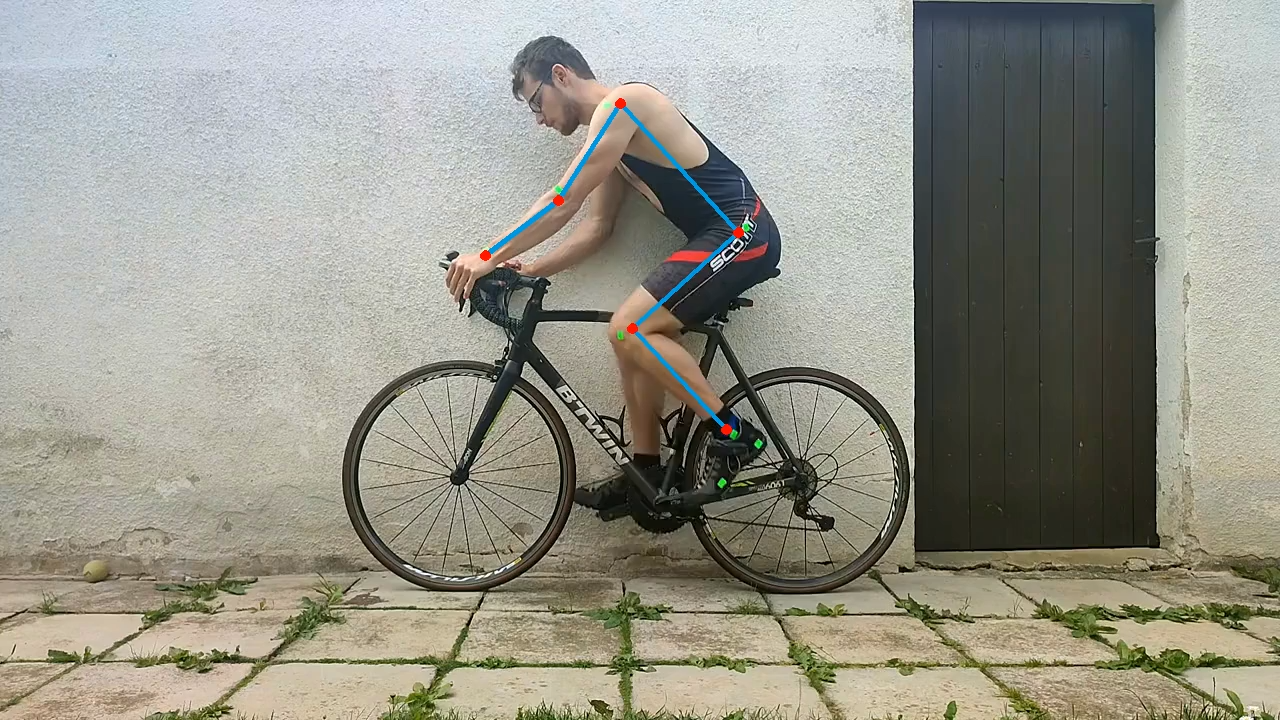
\includegraphics[width=\textwidth]{obrazky-figures/myvelofit_keypoints.png}
    \caption{Side view image with predicted keypoints in MyVeloFit.}
    \label{fig:myvelofit_keypoints}
\end{figure}

From the joint angles for every frame, some are selected for computing the joint angles at the top of the pedal stroke, front of the pedal stroke and bottom. Every position uses different angle ranges and even which angles are taken into account.

\begin{figure}[htbp]
    \centering
    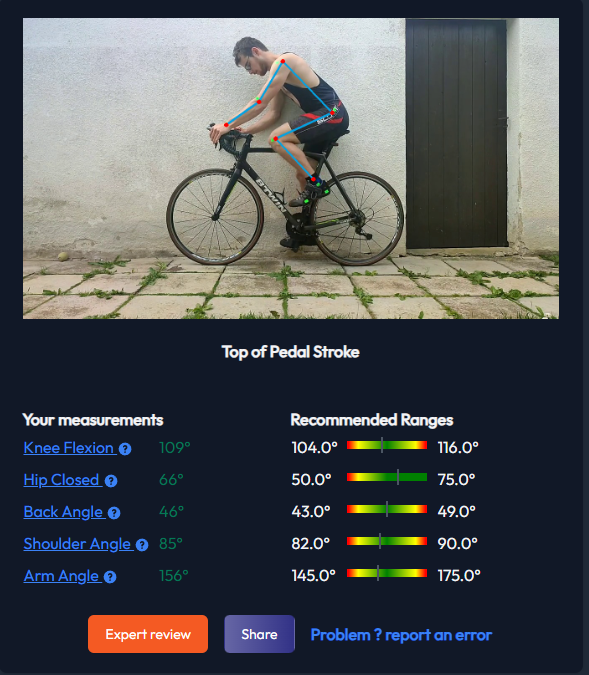
\includegraphics[width=\textwidth]{obrazky-figures/myvelofit_top.png}
    \caption{Predicted joint angles at the top of the pedal stroke in MyVeloFit.}
    \label{fig:myvelofit_top}
\end{figure}

Based on the angles computed for parts of the pedal stroke, MyVeloFit then makes suggestions for saddle height, saddle fore and aft, handlebar height and handlebar reach.

\begin{figure}[htbp]
    \centering
    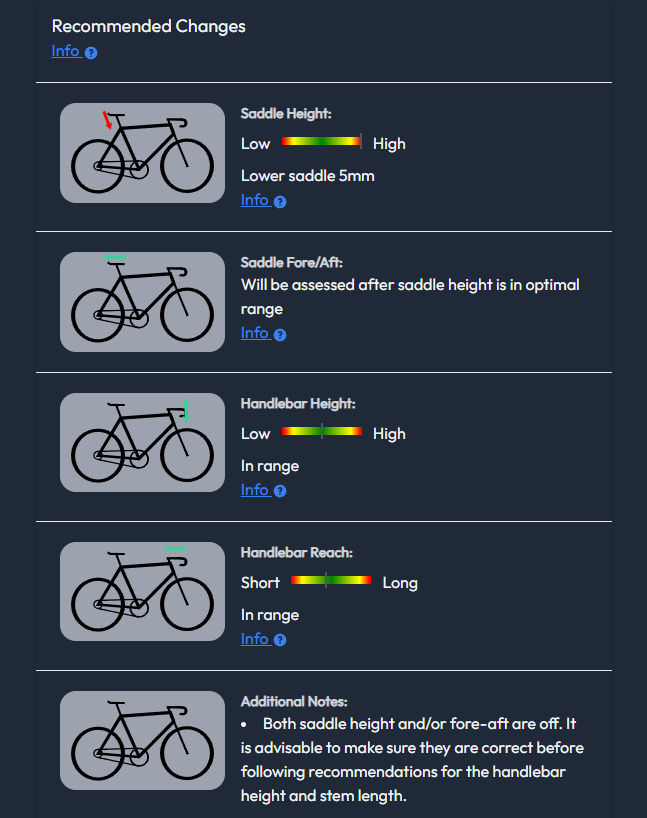
\includegraphics[width=\textwidth]{obrazky-figures/myvelofit_suggestions.png}
    \caption{Recommended changes to the bike position based on the angles computed by MyVeloFit.}
    \label{fig:myvelofit_suggestions}
\end{figure}

Overall, MyVeloFit is relatively easy to use and its joint predictions are fairly accurate. However, it has few disadvantages:

\begin{itemize}
    \item Only the most basic keypoints are used.
    \item Every video is converted to 30 FPS and cut down to 10 seconds.
    \item Video processing and keypoint predictions are slow (3-5 minutes).
    \item Requires subscription to get joint angles and recommended changes. Either a one time payment of 35 US dollars for access for 1 person and 1 bike for 2 weeks or 75 US dollars annually for unlimited number of bikes and people.
\end{itemize}


\subsection{Retul}
\href{https://www.retul.com/}{Retul} is a bike fitting system employing 3D motion capture technologys. It utilizes infrared LED markers placed on specific body points to track the rider's movements dynamically while cycling. The led markers are tracked by multiple infrared cameras placed around the rider. The cameras surprisingly capture only 18 frames per second. Despite this research \cite{retulReliability} shows that the system is relatively reliable compared to 3d motion capture systems with higher frame rates.

Retul uses 8 markers placed on both sides of the rider's body. These markers are placed on the following locations:

\begin{itemize}
    \item Fifth metatarsal of the foot
    \item Heel
    \item Ankle
    \item Knee
    \item Hip
    \item Shoulder
    \item Elbow
    \item Wrist
\end{itemize}

The markers are placed by the fitter on the rider's body. Accurate placement of the markers is crucial for the system to work properly. Even small deviations can lead to inaccurate results.

\begin{figure}[htbp]
    \centering
    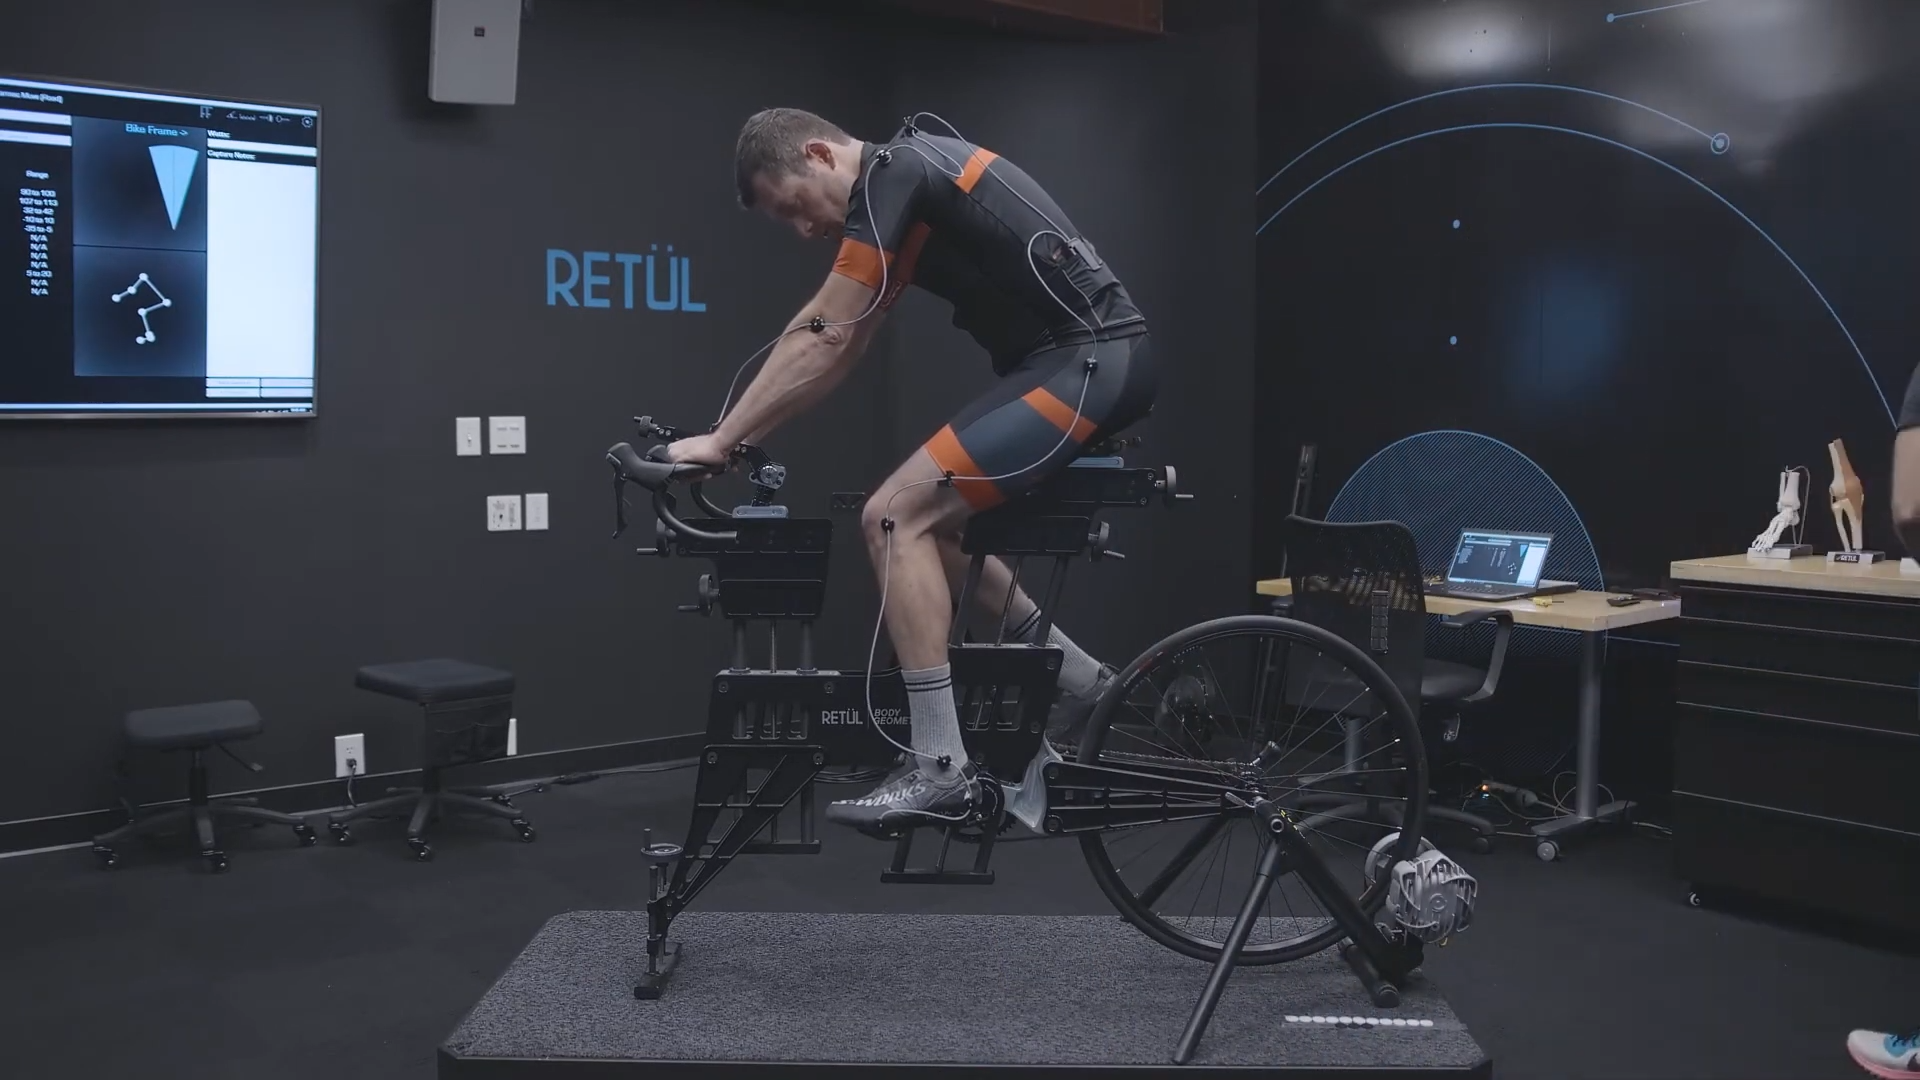
\includegraphics[width=\textwidth]{obrazky-figures/retul_markers.png}
    \caption{Placement of the markers used by Retul.}
    \label{fig:retul_markers}
\end{figure}

Retul's fitting process involves setting up the bike on a trainer equipped with the system. During the session, the rider performs various motions and pedal strokes while the Retul system captures real-time data on joint angles and movements.

Data Captured by Retul includes a wide range of joint angles and movements such as knee angles at top of the pedal stroke and bottom of the pedal stroke, hip angles throughout the pedal stroke, shoulder, elbow, and wrist positions in relation to handlebar reach and drop, as well as ankle and foot movement concerning cleat positioning and alignment.

\begin{figure}[htbp]
    \centering
    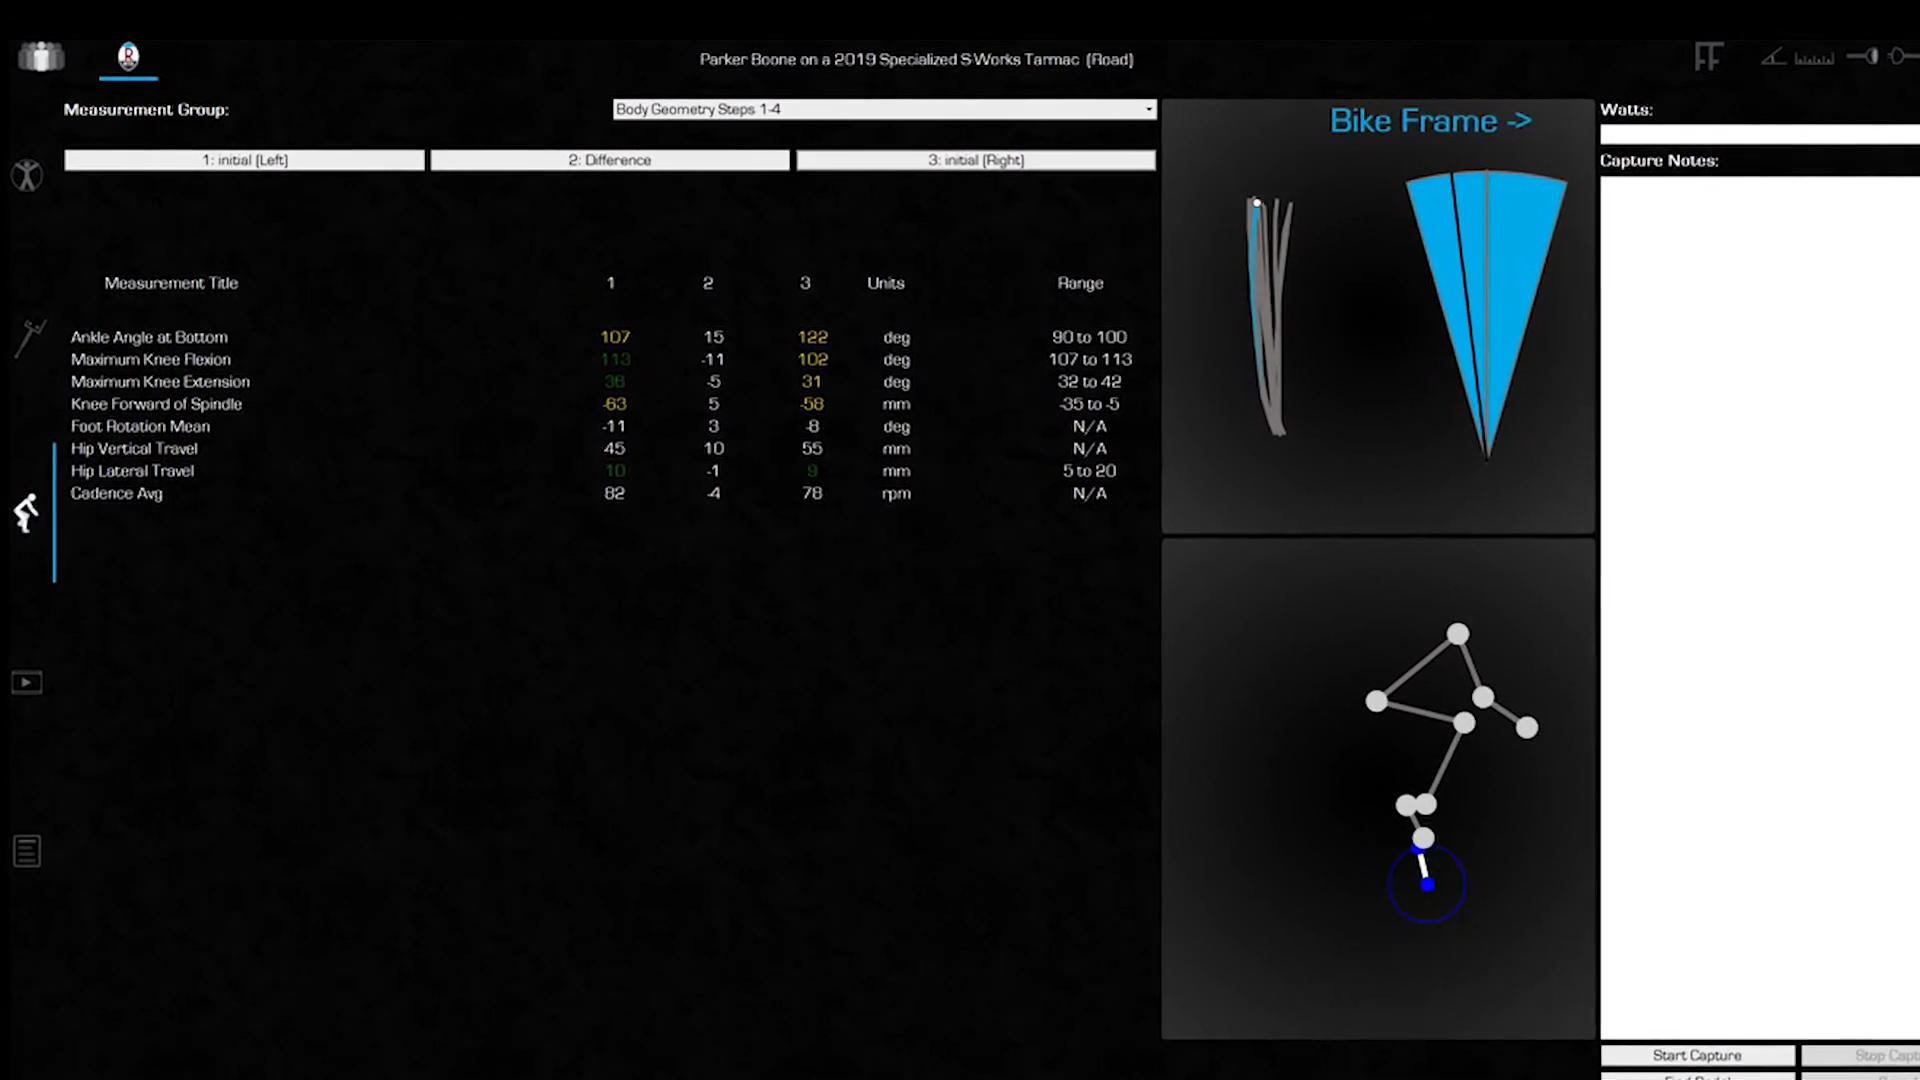
\includegraphics[width=\textwidth]{obrazky-figures/retul_app.png}
    \caption{Retul's software showing the captured data.}
    \label{fig:retul_app}
\end{figure}

The normal ranges for these angles were constructed based on the data collected from thousands cyclists. However, these cyclists were not necessarily optimally fitted to their bikes. Therefore, the normal ranges may not be based on the optimal position for the rider.

Based on the captured data, Retul compares the rider's position to the normal ranges. Based on this comparison, the fitter can make changes to the bike position.

Despite the fact that Retul is a very popular bike fitting system, it has some important disadvantages:
\begin{itemize}
    \item Costly equipment and setup requirements, limiting accessibility to some individuals or smaller bike shops.
    \item The need for trained Retul bike fitters to interpret and implement fitting recommendations effectively.
    \item Requires in-person fitting sessions. These sessions can be time-consuming and costly.
\end{itemize}


\subsection{BikeFast Fit Elite}
\href{https://www.bikefastfit.com/}{BikeFast Fit Elite} is an iOS and Mac OS application that uses pose estimation model to predict the joint locations for a side view video of the user pedaling their bike on an indoor trainer. Compared to MyVeloFit, it uses additional keypoints for the fifth metatarsal of the foot and the heel.

\begin{figure}[htbp]
    \centering
    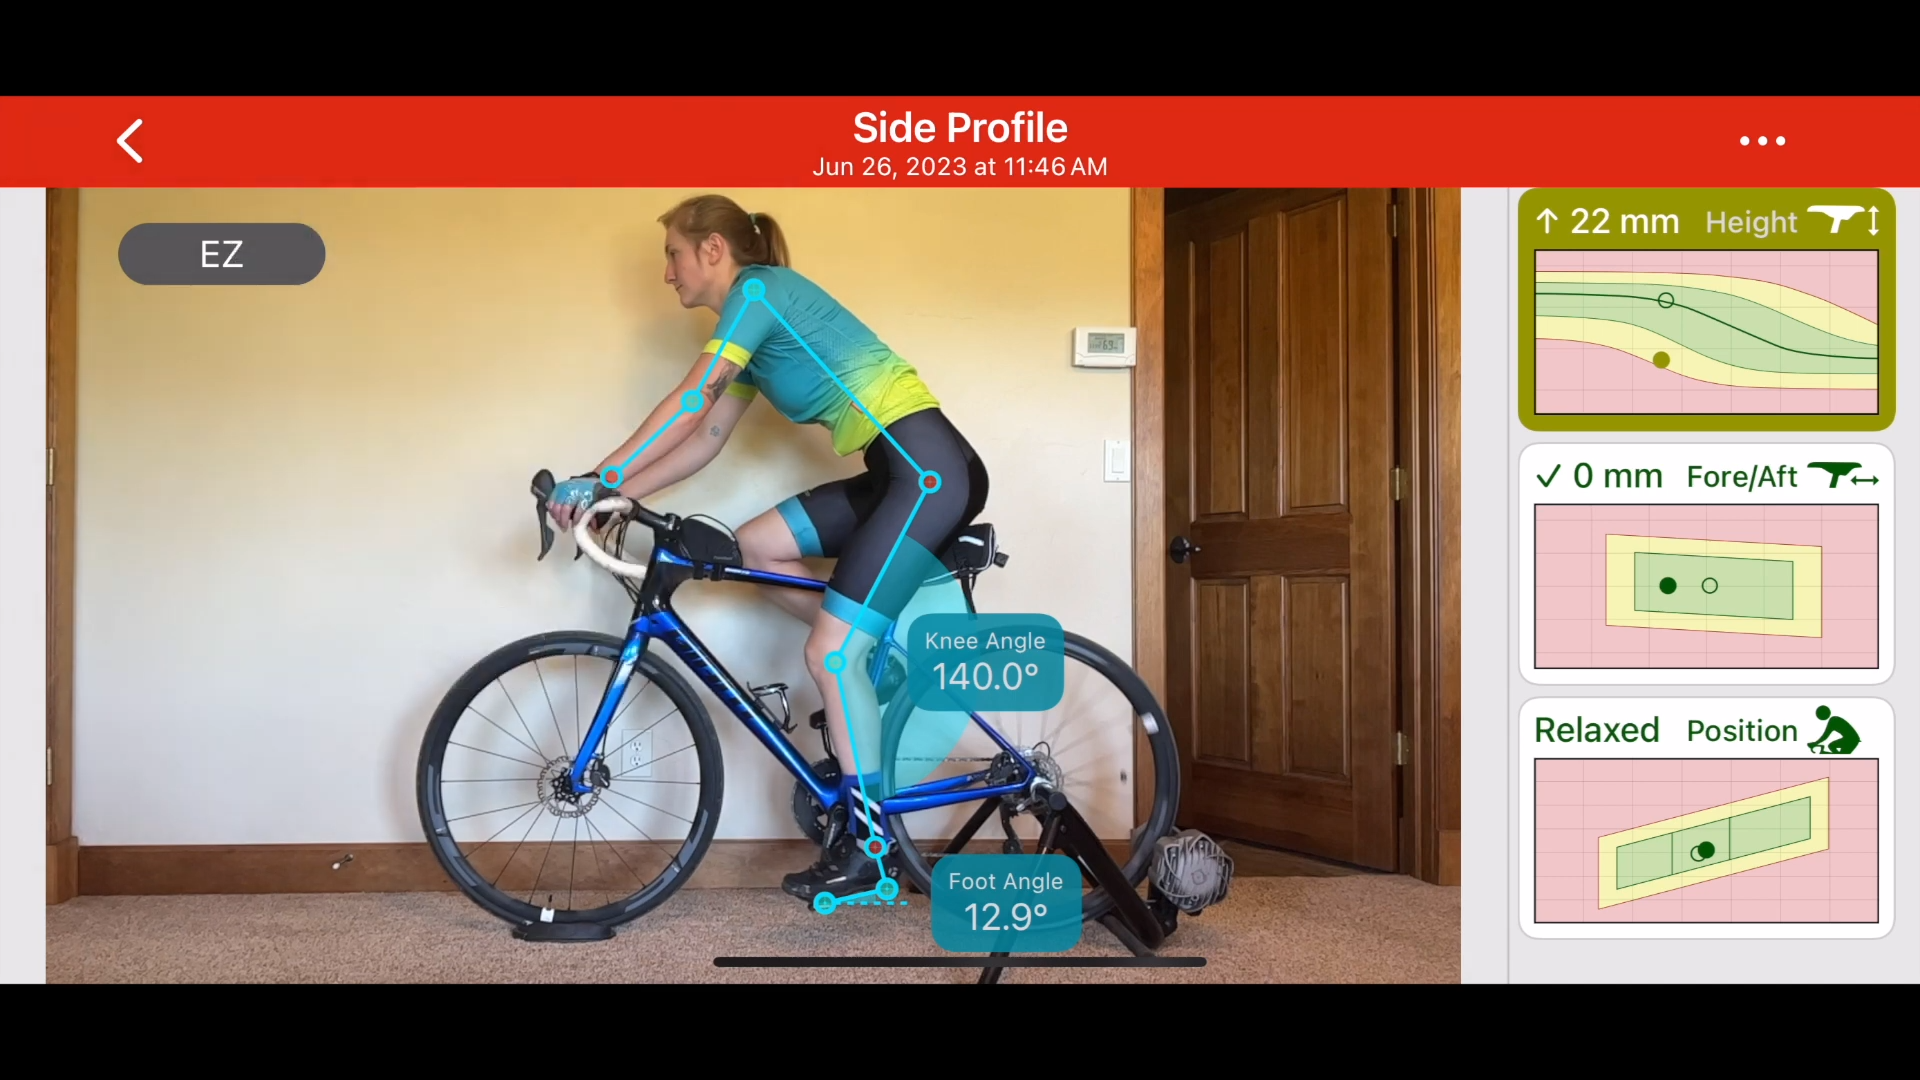
\includegraphics[width=\textwidth]{obrazky-figures/bike_fast_fit_elite.png}
    \caption{Side view image with predicted keypoints in BikeFast Fit Elite.}
    \label{fig:bikefastfit_keypoints}
\end{figure}

Similarly to MyVeloFit, it suggest changes to the saddle height and fore and aft position but it does not suggest changes to the handlebar position, arguing that the handlebar position is based on individual goals and flexibility.

Additionally, it also provides front view knee tracking to address possible knee wobble and asymmetry.

The app costs 19.99 US dollars and does not require a subscription. However, it is only available for iOS and Mac OS. Also it only captures 3.5 seconds of video.


\subsection{Kinovea}


\subsection{Posiclist}



%%%%%%%%%%%%%%%%%%%%%%%%%%%%%%%%%%%%%

\chapter{Pose estimation algorithms}

\section{RTMPose}

\section{Mediapipe}

\section{Evaluation}

\section{Comparison to marker based system}


%%%%%%%%%%%%%%%%%%%%%%%%%

\chapter{Pose estimation dataset for bikefitting}

%%%%%%%%%%%%%%%%%%%%%%%%%%%%%%%%%%%%%%

\chapter{Architechture and implementation of the bikefit application}


\section{Model compression}

\subsection{Group-Fisher pruning}

\subsection{Float16 quantization}

%%%%%%%%%%%%%%%%%%%%%%%%%%%%%%%%%%%%%%

\chapter{Experiments}

%%%%%%%%%%%%%%%%%%%%%%%%%%%%%%%%%%

\chapter{Conclusion}
\label{zaver}

This text summarized the formal requirements for a technical report of a bachelor's thesis or a dissertation. It described the usual procedures used when writing a text of technical nature and offered additional information and independent useful hints and tips for creation of a technical report of a dissertation. It was also explained that a bachelor's thesis also a~dissertation and needs to be approached as such.

It is necessary to point out that dissertation is a unique individual work, that is developed under the supervision of an experienced expert. Regardless of what this template says, you're only obliged to comply with the official guidelines stated on the faculty web pages. You always need to consider which things in the text above are relevant for a specific dissertation and which are not. Most importantly, you should listen to your supervisor, who understands the given problem the most and is therefore able to provide the best advice that you can get.

Despite the effort, it is not possible to include all the elements needed for developing a thesis in this template and guarantee that once the text, images, literature and others are added, that everything will be alright for every single dissertation. A longer text than expected will break to two lines, en entry in list of references that the style was not tested with, and in other cases the result can be hardly satisfying. It could require a modification of the template to account for an error that occurs once in hundred projects. The final PDF and consequently the printed version needs to be thoroughly checked, don't let thoughs like \uv{this was generated by the template, therefore it must be correct} cloud your judgement. If you find errors in the template or you have suggestions on how to improve it, contact us via email at \texttt{sablona@fit.vutbr.cz} and help us improve it. Any and all comments and suggestions are welcome.

Your supervisor can help you significantly when it comes to correcting errors. However, do not expect them to read through your work the night before submission deadline. For that reason, it is necessary to have everything ready in advance and consult your supervisor as you write your dissertation. Supervisor's critical viewpoint can allow for a better result and the extra effort will have a positive effect on their evaluation of the work.


Lastly, on behalf of all the authors, I would like to wish everyone currently in development of their own dissertation and those who are getting ready to start developing it a~successful completion and presentation of their work.

%=========================================================================

% For compilation piecewise (see projekt.tex), it is necessary to uncomment it
% \end{document}